% Milestone 1 slides. Build: tectonic reports/milestone1/slides.tex
\documentclass[aspectratio=169,10pt]{beamer}
\usetheme[progressbar=frametitle,numbering=fraction]{metropolis}
\usepackage{polyglossia}
\setmainlanguage{polish}
\usepackage{booktabs}
\usepackage{graphicx}

% Same hues as the EDA figures: ham = blue, spam = orange.
\definecolor{ham}{HTML}{2A78D6}
\definecolor{spam}{HTML}{EB6834}
\definecolor{spamtext}{HTML}{B4451A}
\definecolor{ink}{HTML}{1B1F24}
\setbeamercolor{frametitle}{bg=ink}
\setbeamercolor{progress bar}{fg=spam,bg=ink!20}
\setbeamercolor{title separator}{fg=spam}
\setbeamercolor{alerted text}{fg=spamtext}
\setbeamercolor{block title}{bg=ink!10,fg=ink}
\setbeamercolor{block body}{bg=ink!4}

\newcommand{\ham}{\textcolor{ham}{\textbf{ham}}}
\newcommand{\spam}{\textcolor{spamtext}{\textbf{spam}}}

\title{Wykrywanie spamu w wiadomościach SMS}
\subtitle{Milestone 1}
\author{Jerzy Czarnecki \and Mateusz Małachowski \and Sebastian Rydz \and Wojciech Wójcik}
\date{29.10.2026}

\begin{document}

\maketitle

\begin{frame}{Dane: 5574 SMS-y, 13,4\% spamu}
  \begin{columns}[T]
    \begin{column}{0.34\textwidth}
      \begin{itemize}
        \item SMS Spam Collection v.1\\{\small UCI \#228, CC BY 4.0}
        \item \ham{} 4827 \quad \spam{} 747
        \item braki i puste: \textbf{0}
        \item emoji: \textbf{0} (rok 2011)
        \item 35 SMS-ów z błędnym cp1252
        \item \texttt{id} = nr linii pliku
      \end{itemize}
      \vspace{0.6em}
      \textbf{Metryka główna:}\\F1 dla klasy spam
    \end{column}
    \begin{column}{0.64\textwidth}
      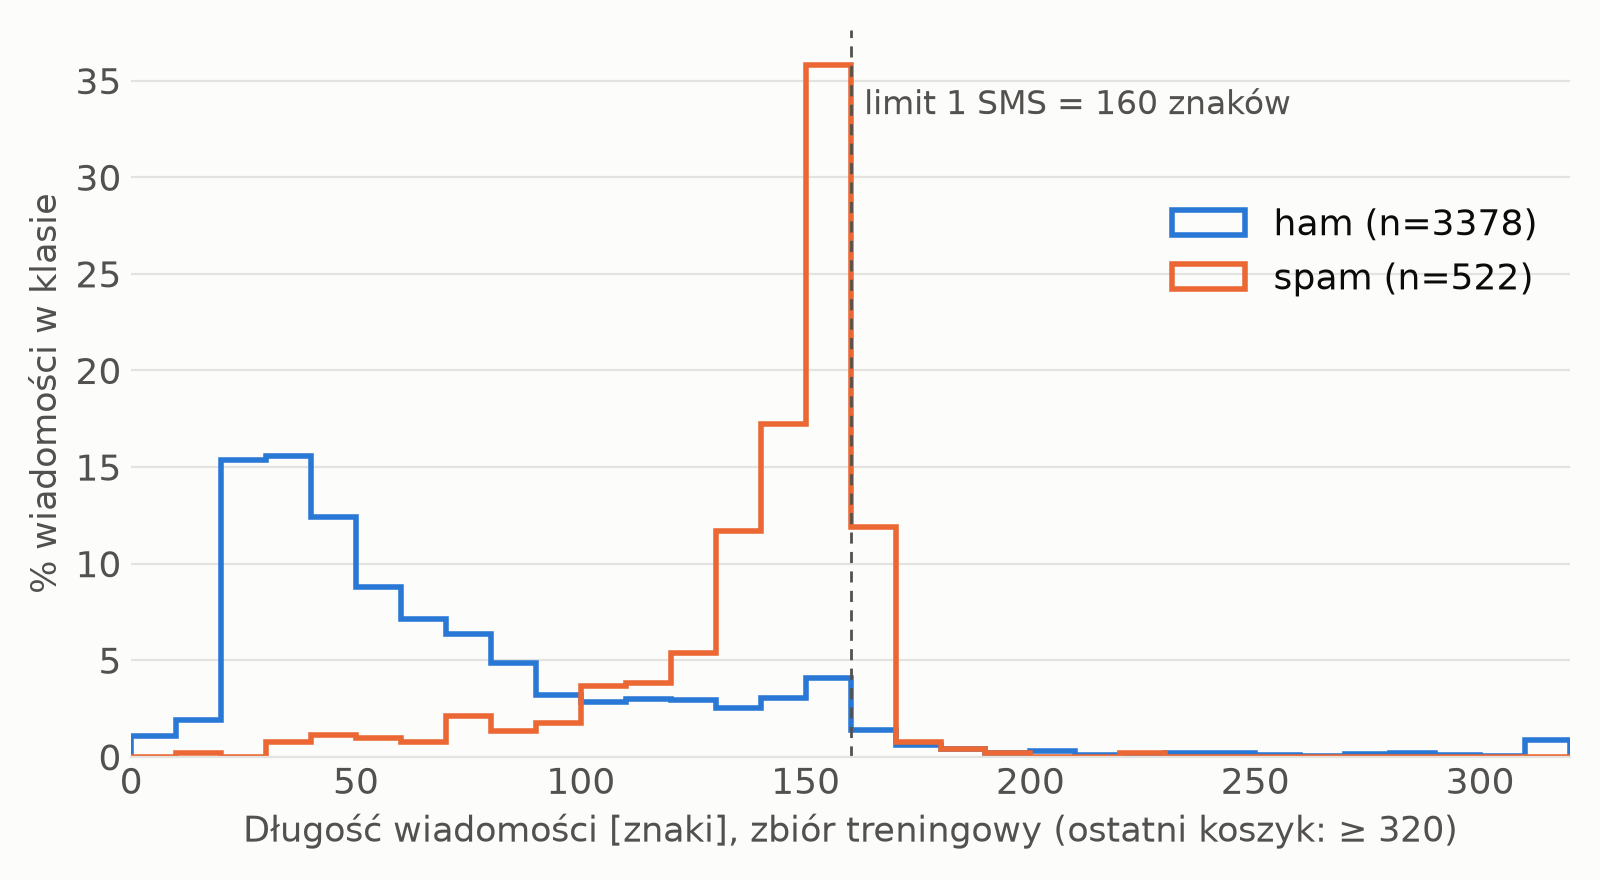
\includegraphics[width=\linewidth]{fig_length.png}\\[0.2em]
      {\small Spam celuje w limit jednego SMS-a: mediana \textbf{149} znaków (ham: 53),
      74,7\% spamu ma 120--160 znaków.}
    \end{column}
  \end{columns}
\end{frame}

\begin{frame}{Duplikaty i podział bez przecieku}
  \begin{columns}[T]
    \begin{column}{0.5\textwidth}
      \begin{itemize}
        \item \textbf{403} dokładne duplikaty (7,2\%);\\spam powtarza się 2× częściej (12,6\% vs 6,4\%)
        \item \textbf{0} tekstów z konfliktem etykiet
        \item Bliskie duplikaty: cosinus TF-IDF n-gramów znakowych 3--5 $\geq$ 0,7, czyli 4897 grup (największa: 40).
          Najczęściej ten sam szablon spamu z innym numerem.
        \item Decyzja: zostawiamy wszystkie rekordy, a każda grupa trafia w całości do jednej części.
      \end{itemize}
    \end{column}
    \begin{column}{0.46\textwidth}
      \centering
      \begin{tabular}{lrrrr}
        \toprule
        część & ham & spam & razem & \% spam \\
        \midrule
        train & 3378 & 522 & 3900 & 13,4 \\
        val   &  725 & 112 &  837 & 13,4 \\
        test  &  724 & 113 &  837 & 13,5 \\
        \bottomrule
      \end{tabular}\\[0.8em]
      {\small 70/15/15, StratifiedGroupKFold, seed 42}
    \end{column}
  \end{columns}
\end{frame}

\begin{frame}{Co odróżnia spam od hamu (zbiór treningowy)}
  \centering
  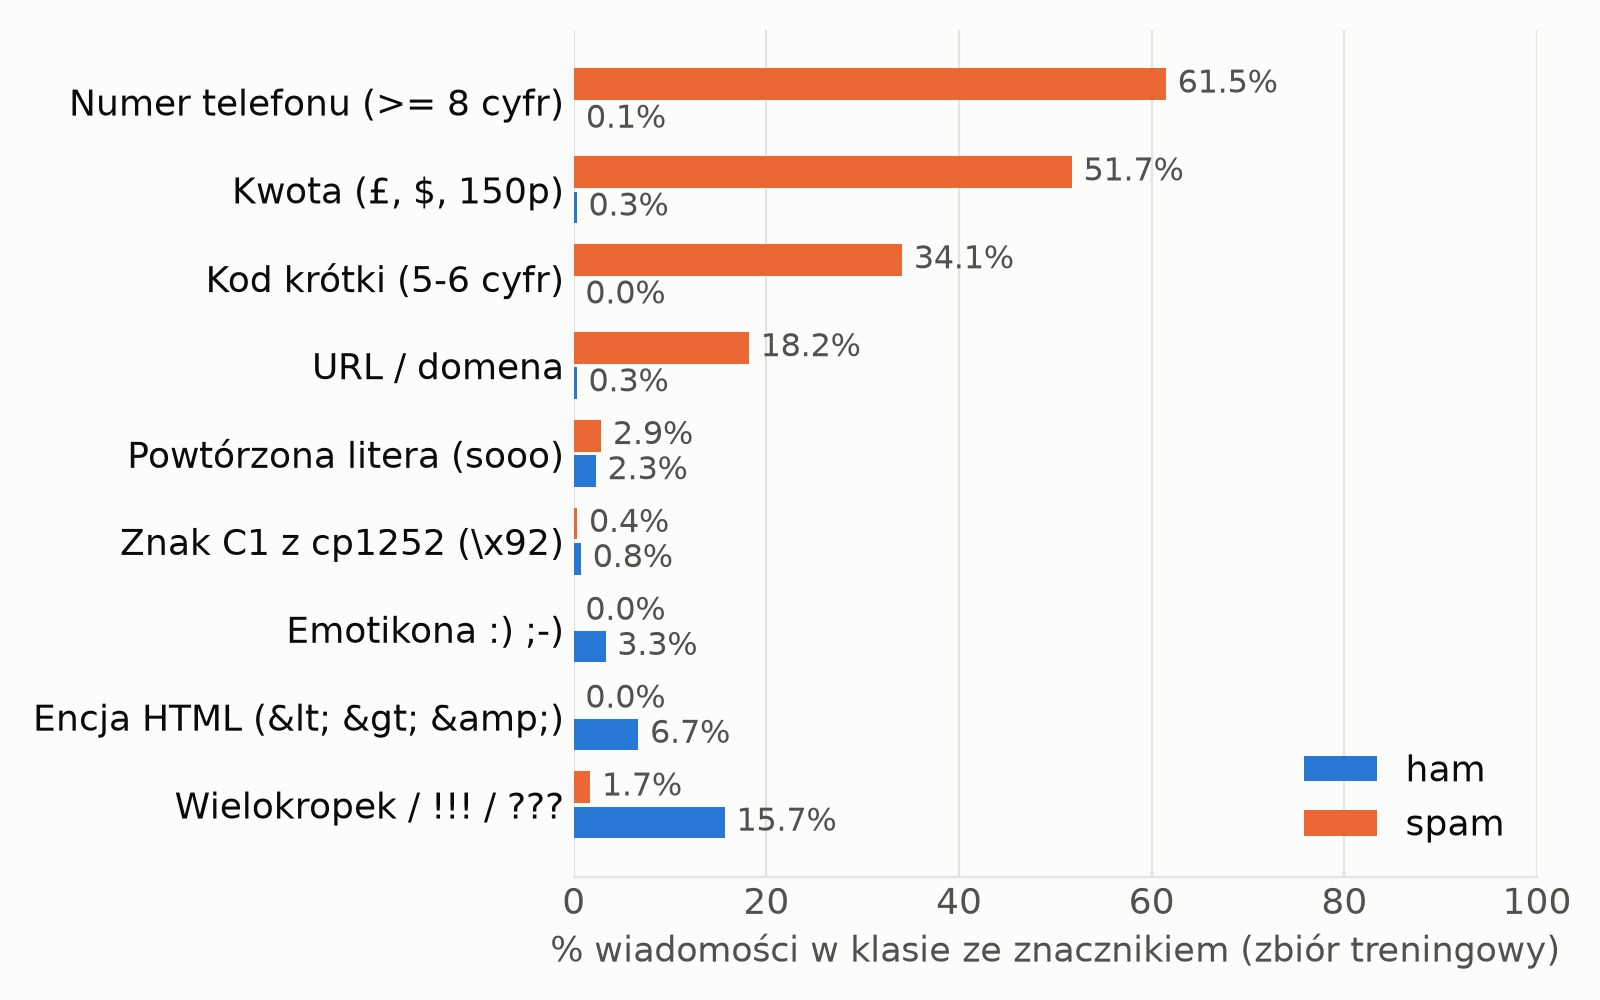
\includegraphics[width=\linewidth,height=0.82\textheight,keepaspectratio]{fig_markers.png}
\end{frame}

\begin{frame}{Trzy hipotezy: ten sam model B1, zmieniamy tylko tekst}
  \small
  \begin{columns}[T]
    \begin{column}{0.32\textwidth}
      \begin{block}{P1: maskowanie numerów i kwot}
        \texttt{<PHONE> <SHORTCODE> <MONEY>}\\[0.4em]
        \textbf{Dlaczego:} numer telefonu w 61,5\% spamu, ale 91\% długich liczb to kolumny BoW z $\leq$ 2 dokumentów.\\[0.4em]
        \textbf{Oczekujemy:} wyższego recall spamu i F1.\\[0.4em]
        \textbf{Ryzyko:} hamy z kwotami (\texttt{\$700}).
      \end{block}
    \end{column}
    \begin{column}{0.32\textwidth}
      \begin{block}{P2: URL, maskowanie vs usuwanie}
        \texttt{<URL>} albo usunięcie\\[0.4em]
        \textbf{Dlaczego:} URL w 18,2\% spamu, ale tokenizer już rozbija domeny (\texttt{uk}: 50 spam / 1 ham).\\[0.4em]
        \textbf{Oczekujemy:} maskowanie bez większej zmiany, usunięcie obniży recall.
      \end{block}
    \end{column}
    \begin{column}{0.32\textwidth}
      \begin{block}{P3: normalizacja powtórzeń}
        \texttt{sooo}$\to$\texttt{soo}, \texttt{!!!!}$\to$\texttt{!!}\\[0.4em]
        \textbf{Dlaczego:} powtórzenia tylko w 2--3\% wiadomości obu klas.\\[0.4em]
        \textbf{Oczekujemy:} braku istotnej zmiany na czystym teście; ewentualny zysk w teście odporności na literówki.
      \end{block}
    \end{column}
  \end{columns}
  \vspace{0.8em}
  Najpierw zmiany pojedyncze, potem połączenie najlepszych.
\end{frame}

\begin{frame}{Problemy i plan na Milestone 2}
  \begin{columns}[T]
    \begin{column}{0.48\textwidth}
      \textbf{Problemy i ryzyka}
      \begin{itemize}
        \item Mały test: 113 spamów, więc 1 SMS $\approx$ 0,9 p.p. recall. Potrzebny sparowany bootstrap.
        \item 65 ze 113 spamów testu jest w grupach duplikatów. Raportujemy też test po deduplikacji (781 unikalnych).
        \item 41 spamów testu przypomina kampanie z treningu (cos 0,5--0,7). Pokażemy wynik na podzbiorze $<$ 0,5.
      \end{itemize}
    \end{column}
    \begin{column}{0.48\textwidth}
      \textbf{Plan M2}
      \begin{itemize}
        \item B0: klasa większościowa (ham), F1 spamu = 0
        \item B1: TF-IDF na surowym tekście (\texttt{lowercase}, domyślny \texttt{token\_pattern}) + regresja logistyczna;
          \texttt{C} i próg decyzji tylko na walidacji
        \item P1--P3 na zamrożonym B1, potem połączenie najlepszych
        \item Osobny eksperyment: n-gramy słowne vs znakowe
      \end{itemize}
    \end{column}
  \end{columns}
\end{frame}

\end{document}
